\chapter{Reconstrução à Laser}\label{cap:laser}

\section*{Introdução}

A técnica de reconstrução baseada em \emph{laser} é conhecida desde o século passado, pois oferecem uma alta qualidade geométrica de dados, os resultados são em tempo real e requer pouco tempo de captura de dados. 
Neste caso, abordaremos o projeto de escaneamento da escultura de Michelangelo, David, que utiliza escaneadores baseados em superfícies, mais especificamente, utilizando uma técnica conhecida como \emph{Time of Flight}, ou tempo de voo \ref{fig:luzestruturada}. Este processo se baseia em projetar um padrão conhecido (muitas vezes, grades ou barras horizontais, via \emph{laser}) em uma cena. A forma como o padrão se deforma quando atinge superfícies permite que sistemas de visão calculem a profundidade e informações das superfícies dos objetos na cena.

\begin{figure}[!h]
	\centering
	%   \includegraphics[width=1.0\linewidth]{figs/3d-curve-sketch/system-diagram.eps}
	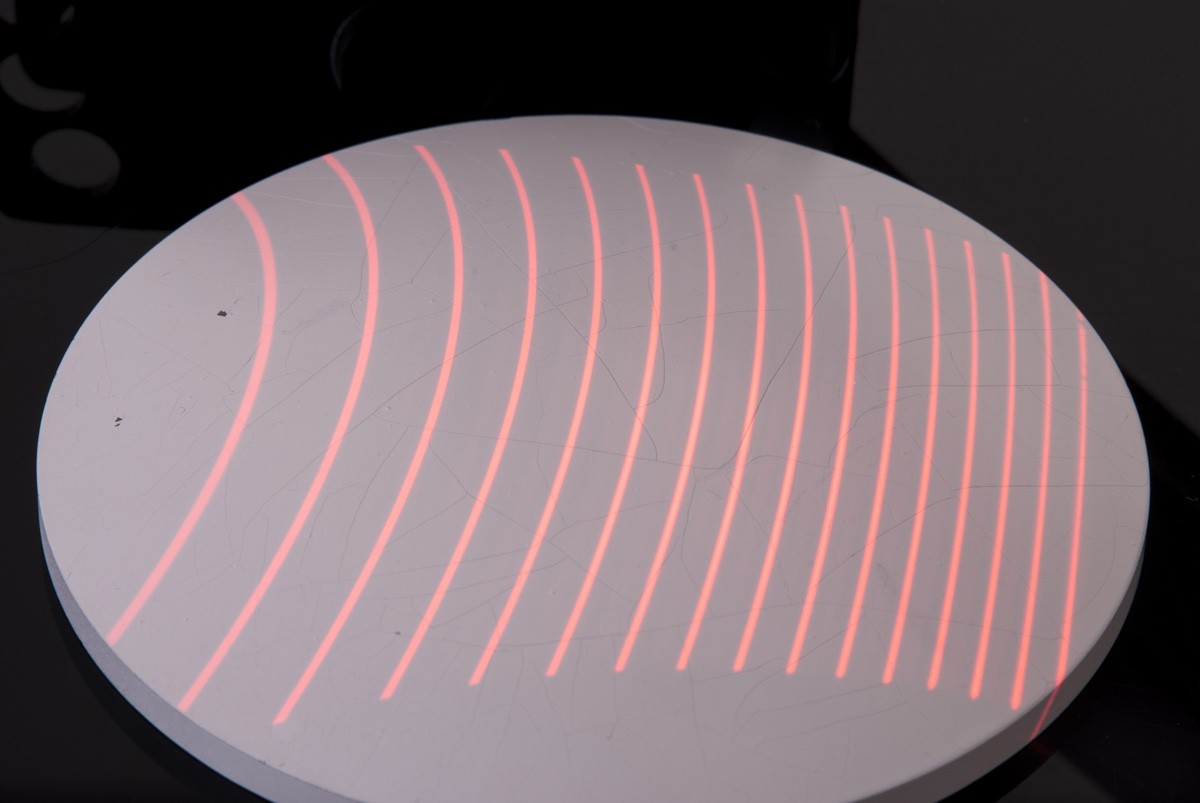
\includegraphics[width=0.7\linewidth]{figs/luzestruturada.jpg}
	\caption{%
	Exemplo de um projetor de padrões utilizando um \emph{laser} visível.
	\cite{luzEstruturada}.
	}\label{fig:luzestruturada}
\end{figure}

\section{Projeto de preservação das esculturas de Michelangelo}\label{sec:David}

\subsection*{Introdução}

Este projeto tem como motivação avançar a tecnologia de digitalização 3D e criar um acervo digital sobre alguns dos principais artefatos culturais. Foram utilizados sensores de alcance (\emph{range finders}) para triangulação, sensores de alcance baseados em ToF (\emph{Time of Flight}), câmeras digitais e um software de calibração. Com uma equipe de mais de 30 professores, funcionários e estudantes da Universidade de Stanford desenvolveram algoritmos para combinar imagens de múltiplas gamas e cores, passaram os anos de 1998 e 1999 na Itália escaneando esculturas de Michelangelo. 

O principal componente de hardware do sistema é um escaneador de triangulação a \emph{laser}, que é composto por 4 eixos motorizados, um \emph{laser}, uma câmera de alcance, uma câmera de cores e uma luz branca~\ref{fig:cabecaScanner}, isso tudo acrescido de suportes e estruturas para o escaneamento de estátuas grandes. O objetivo de um escaneador deste porte era capturar marcas menores que um milímetro, das ferramentas utilizadas por Michelangelo em suas esculturas. 
Para isso foram testadas diversas resoluções, na qual foi decidido um espaçamento Y (ao longo da faixa do \emph{laser}) de 1/4 mm e uma resolução Z (profundidade) de pelo menos duas vezes este valor. 
O que resultou em uma visualização de 14 cm de largura (ao longo da faixa do \emph{laser}) por 14 cm de profundidade. Caso esta resolução fosse menor, as marcas de cinzelão ficariam borradas e se fosse maior, o conjunto de dados produzido seria gigantesco.
Felizmente, a maioria das estátuas feitas por Michelangelo foram esculpidas com um mármore encontrado em Carrara Statuario, uma pedra altamente uniforme, não direcional e constituída de grãos finos. Além disso, com exceção da "Noite"~\ref{fig:noite}, as esculturas não são polidas e cobertas por terra, o que aumenta a dispersão superficial e reduz a abaixo da superfície.
Neste contexto, a dispersão abaixo da superfície causa alguns problemas: não se pode assumir que a superfície é Lambertiana ideal~\cite{basri2003lambertian}, mudou a forma com que a renderização dos modelos seriam feitos e diminuiu a qualidade de disposição de dados.

\begin{figure}[!h]
	\centering
	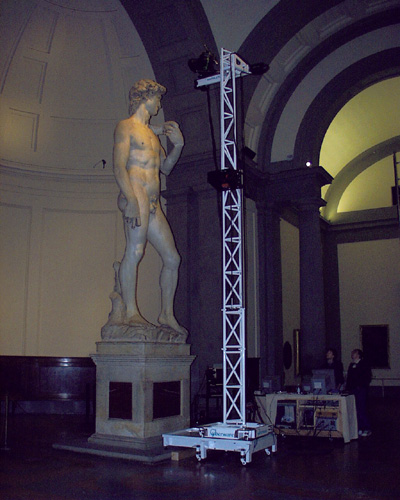
\includegraphics[width=0.3\linewidth]{figs/gantry-and-david4-s.jpg}(a)
	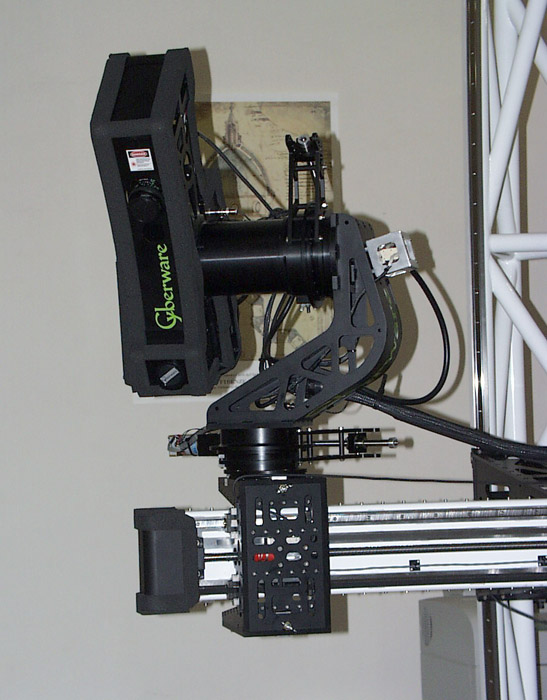
\includegraphics[width=0.3\linewidth]{figs/mgantry-scannerhead-s.jpg}(b)
	\caption{%
	Como era feito o escaneamento da estátua de David (a), composto por dois escaneadores, sendo (b) o escaneador principal (da cabeça) e estruturas para alcançar todos os pontos necessários.
	\cite{levoy2000digital}.
	}\label{fig:cabecaScanner}
\end{figure}

\begin{figure}[!h]
	\centering
	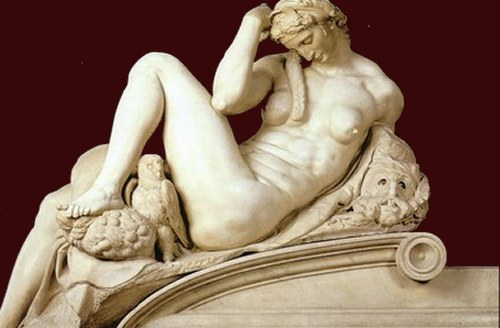
\includegraphics[width=0.4\linewidth]{figs/michelangelo-notte.jpg}
	\caption{%
	Escultura "Noite", de Michelangelo.
	}\label{fig:noite}
\end{figure}

\subsection*{Calibração}

O objetivo de calibrar o aparato era encontrar um mapeamento de coordenadas 2D no seu alcance e cores para coordenadas 3D em um quadro de referência global. Idealmente, este quadro deve ser a estátua (estacionária). Porém não foi rastreado o aparato, ele tornou-se a própria referência. O mapeamento final foi realizado alinhando novas varreduras, com varreduras previamente existentes.

Para calibrar qualquer sistema, primeiramente escolhe-se um modelo matemático que se aproxime do comportamento do sistema, então estima-se parâmetros desse modelo medindo o comportamento do sistema. No caso do projeto de David, o modelo matemático natural era um modelo geométrico 3D parametrizado da cabeça digitalizada e do aparato. Se os componentes do sistema forem suficientemente independentes, a calibração pode ser dividida em estágios, correspondente a cada componente do sistema. Por isso o aparato foi construído pensando na rigidez (independência), pois particionar a calibração em etapas reduz o grau de liberdade em cada etapa, e com isso, o número de medidas necessárias para calibrar este estágio.

Em um sistema mecânico, também é reduzido o volume físico total na qual essas medidas de calibração devem ser tomadas. Além disso, uma calibração em etapas é menos suscetível a propagação de erros, pois caso uma calibração falhasse, seria apenas uma parte da calibração e não o sistema como um todo. No projeto de David, a calibração foi divida em seis etapas distintas:

\begin{enumerate}
\item{Um mapeamento 2D a partir de coordenadas de \emph{pixels} das imagens da câmera para locais físicos na camada de laser}
\item{Transformação rígida 2D/3D do sistema de coordenadas da camada do \emph{laser} para esferas de aço anexadas ao escaneador da cabeça}
\item{Transformação rígida 3D para acomodar o rolamento do escaneador da cabeça em $90^{\circ}$ (ao remontá-lo) em relação ao conjunto de inclinação}
\item{A localização do eixo de rotação de inclinação e o mapeamento não-linear de movimento comandos para ângulos de rotação físicas}
\item{A localização do eixo de rotação panorâmico e o mapeamento de seus comandos de movimento para ângulos de rotação física}
\item{A localização do eixo de translação, que também depende de como o conjunto inclinação-panorâmico está montado no braço horizontal}
\end{enumerate}

O resultado da calibração pode ser descrito como uma concatenação de seis matrizes 4x4:
\[
\begin{bmatrix}
\text{translação} \\ 
\text{horizontal}
\end{bmatrix}
\begin{bmatrix}
\text{rotação} \\ 
\text{panorâmica}
\end{bmatrix}
\begin{bmatrix}
\text{rotação} \\
\text{de} \\
\text{inclinação}
\end{bmatrix}
\begin{bmatrix}
\text{rotação} \\
\text{de} \\
\text{rolamento}
\end{bmatrix}
\begin{bmatrix}
\text{laser para o} \\
\text{escaneador }
\text{da cabeça}
\end{bmatrix}
\begin{bmatrix}
\text{imagem} \\
\text{para o} \\
\text{laser}
\end{bmatrix}
\]

% Calibração do sistema de cores:
% Para corrigir a distorção geométrica na câmera de cores, foi fotografado um alvo de calibração planar que possui um certo número de \emph{features} que, por sua vez, foram usados para calcular os parâmetros intrínsecos da câmera. Estão inclusos no modelo dois termos de distorção radial e dois termos de distorção tangencial que tem uma projeção de perspectiva fora do centro e uma escala possivelmente não uniforme (em X e Y) %CITAR[Heikkila..97].%

% Para obter um mapeamento da câmera colorida para o escaneador da cabeça, o alvo foi escaneado usando o \emph{laser} e a câmera de alcance. Uma vez que o escaneador retornou a intensidade refletida pelo \emph{laser}, bem como a profundidade, pode-se calcular as coordenadas 3D de cada ponto da \emph{feature}.

% Para corrigir os efeitos radiométricos espaciais, incluindo o aspecto de vinheta das lentes, a não uniformidade angular, o declínio da lei quadrada inversa dos holofotes e a não uniformidade espacial na resposta do sensor, foi fotografado um cartão branco sob o holofote e construída uma tabela de correção de intensidade por pixel.

% Depois de testar várias resoluções, decidimos um espaçamento de amostra Y (ao longo da faixa \emph{laser}) de 1/4 mm e uma resolução Z (profundidade) pelo menos duas vezes esta multa 1. Isso nos deu uma visão de 14 cm de largura (ao longo da faixa a \emph{laser} ) por 14 cm de profundidade. Em retrospectiva, ficamos satisfeitos com a resolução que escolhemos; Qualquer coisa menor teria significativamente borrado as marcas de cinzelão de Michelangelo, e qualquer coisa maior teria tornado os nossos conjuntos de dados não gerenciáveis.

\begin{figure}[!h]
	\centering
	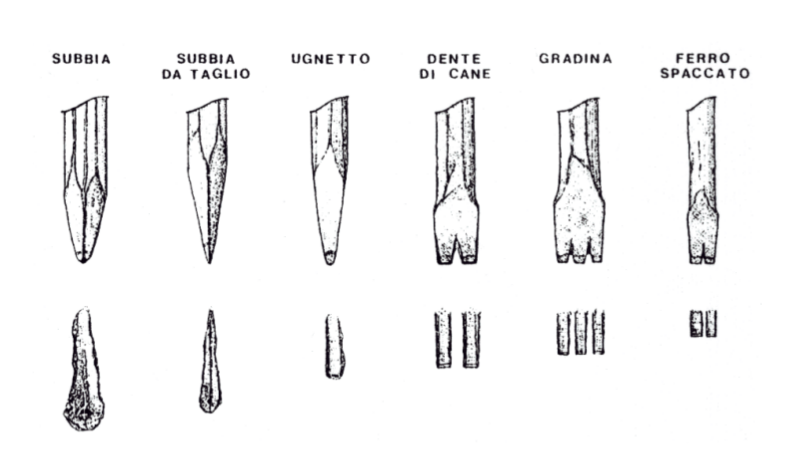
\includegraphics[width=0.5\linewidth]{figs/ferramentasMich.png}
	\caption{%
	Alguns tipos de cinzelões que provavelmente foram usados por Michelangelo na escultura de "St. Matthew".
	\protect\cite{levoy2000digital}.
	}\label{fig:noite}
\end{figure}

\subsection*{Procedimento de digitalização}

Um operador move, interativamente o escaneador da cabeça através de uma sequência de movimentos, definindo os limites de volume a ser escaneado. O volume que pode ser coberto em uma única varredura, foi delimitado por conta de quatro fatores:
\begin{itemize}
\item{O campo de visão e os limites de movimento do escaneador}
\item{A  queda na qualidade da varredura com o aumento da obliquidade do laser}
\item{Oclusões, tanto do \emph{laser} quanto da linha de visão da câmera}
\item{Obstruções físicas, como paredes, estátuas ou o próprio equipamento}
\end{itemize}

Uma vez planejada a varredura, um script de digitalização é executado automaticamente, levando desde alguns minutos, até horas para terminar, dependendo da largura da área a ser coberta.
A partir do script, são feitas as etapas de escaneamento de alcance (\emph{laser}) e do escaneamento colorido (câmera digital).

% Range scanning. A typical range scan consisted of several con-
% centric curved shells separated by translational motion of the scan
% head along the horizontal table. Each shell in turn consisted of sev-
% eral horizontally adjacent vertical sweeps of the \emph{laser}, as shown in
% figure 5. If the \emph{laser} line was turned vertically, then the sweeps were
% horizontal instead. We decided to overlap adjacent sweeps and
% shells by 40% and 15%, respectively - enough to align them in soft-
% ware in the absence of precisely calibrated motion. Since scanning
% was slow (1 cm per second), we preceded each sweep with a high-
% speed (10 cm per second), low-resolution pre-scan that conserva-
% tively determined which part of the sweep actually contained data.

%Alcance da varredura
% Escala de varredura. Uma varredura de varredura típica consistiu em vários reservatórios curvos concêntricos separados pelo movimento de translação da cabeça de varredura ao longo da mesa horizontal. Cada casca, por sua vez, consistiu em vários varredões verticais horizontais adjacentes do \emph{laser}, como mostrado na figura 5. Se a linha do \emph{laser} foi girada verticalmente, então os varreduras estavam em vez da horizontal. Decidimos sobrepor as varreduras e os reservatórios adjacentes em 40% e 15%, respectivamente - o suficiente para alinhá-los no software na ausência de movimento calibrado com precisão. Uma vez que a varredura foi lenta (1 cm por segundo), precedemos cada varredura com uma pré-digitalização de alta velocidade (10 cm por segundo) e de baixa resolução que determinou de forma conservadora qual parte da varredura realmente continha dados.

% O principal componente de hardware do nosso sistema foi um escaneador de triangulação a \emph{laser} e um pórtico motorizado personalizado para digitalizar grandes estátuas. Nossos requisitos para este escaneador eram exigentes; queríamos capturar marcas de cinzelão menores do que um milímetro, queríamos capturá-las a uma distância segura, e queríamos chegar ao topo do David de Michelangelo, que tem 23 pés de altura no pedestal. Nas seções que se seguem, descrevemos os sistemas de aquisição de alcance e cor deste escaneador, seu pórtico mecânico de suporte e nosso procedimento para calibrá-lo.

Primeiramente faz-se o escaneamento da geometria da escultura:

\begin{itemize}
\item{Alinhamento manual}
\item{ICP -- \emph{Iterative Closest Point} para uma câmera existente} %CITAR ICP AQUI%
\item{ICP automático para todos os pares sobrepostos}
\item{Relaxação global para espalhar o erro}
\item{Reunir utilizando métodos volumétricos}
\end{itemize}


Após isso, ocorre o escaneamento e processamento das cores da escultura:

\begin{itemize}
\item{Compensação da iluminação do ambiente}
\item{Descarte de pixels com sombra ou especulares}
\item{Mapeia-se os vértices (uma cor por vértice)}
\item{Correção da irradiância e reflectância difusa}
\end{itemize}

Limitações:
\begin{itemize}
\item{Inter-reflexões são ignoradas}
\item{Dispersões subterrâneas são ignoradas}
\item{Tratamento difuso com Lambertiano} %CITAR TREATED DIFFUSED AS LAMBERTIAN%
\item{Usa superfícies normais agregadas}
\end{itemize}

O projeto não teve mais nenhum avanço desde o verão de 2004, por falta de financiamento. Como resultado, modelos de alta qualidade só existem do David na resolução de 1,0 mm (56 milhões de triângulos) e São Mateus a 0,25 mm (372 milhões de triângulos). Um modelo também existe para o Atlas em 0,25 mm (aproximadamente 500 milhões de triângulos), mas contém erros de alinhamento. Após 6 anos de trabalho estudantil remunerado e voluntário, existem modelos para cada um dos 1.186 fragmentos. Esses modelos, que totalizam quase 8 bilhões de polígonos, se encontram no próprio site da Universidade de Stanford %CITAR AQUI$. 

Também foram disponibilizadas algumas métricas sobre este projeto \ref{tab:metricasDavid}.

\begin{table}
\caption{Métricas do projeto de reconstrução da escultura David}
\label{tab:metricasDavid}
\begin{tabular}{|l|p{4.7cm}|}
\hline
Números de objetos escaneados          & 10 estátuas + 2 edificações + 1.163 fragmentos de mapa  \\ \hline
Menor e maior objetos escaneados       & 1 polegada (fragmentos de mapa) e 23 pés (David)         \\ \hline
Resolução espacial dos dados                & 0,29mm para geometria, 0,125mm para cor              \\ \hline
Complexidade do maior conjunto de dados             & 2 bilhões de polígonos + 7.000 imagens (David)\\ \hline
Tamanho do maior conjunto de dados                    & 32 \emph{gigabytes} (David)                  \\ \hline
Quantia total de dados capturados              & 250 \emph{gigabytes}                                 \\ \hline
Tamanho do maior escaneador                    & 24 pés de altura, 1.800 libras de peso                  \\ \hline
Peso total do equipamento levado para a Itália & 4 toneladas                                              \\ \hline
Número de pessoas envolvidas                  & 32 (sem incluir subcontratantes e colaboradores) \\ \hline
Tempo médio para escaneamento              & 1 semana (exceto o David, que levou 1 mês)       \\ \hline
Tempo total de escaneamento                 & 5,.00 horas de trabalho                                   \\ \hline
Total de tempo para processamento de dados          & 4.000 horas de trabalho (até agora)                            \\ \hline
Custo do projeto                          & \$2.000.000                                         \\ \hline
\end{tabular}
\end{table}


Porém, devido ao seu alto custo com equipamentos, com softwares e sem falar na necessidade de estações robustas para armazenamento dos dados e para escaneamento de patrimônios, outras técnicas foram emergindo com o passar dos anos, como a fotogrametria, que será abordada ao decorrer deste documento.

% \chapter{Kinect}\label{sec:kinect}
%======================================================================================
Um componente criado pela Microsoft para fins recreativos (como no XBox, por exemplo), virou uma das mais conhecidas ferramentas de reconstrução 3D no cenário atual. Sua primeira versão (Kinect V1) utiliza uma técnica similar à empregada no projeto da Universidade de Stanford, com luz estruturada, porém, diferentemente dos escaners à laser, o Kinect tem um custo monetário baixo e é acessível a todo público em geral (desde entusiastas, amadores até profissionais da área). 

O Kinect V2 utiliza uma projeção de fótons [...] e por isso ele já não é tão utilizado na área de reconstrução 3D como o V1. 

O V1 é composto por 2 câmeras: uma RGB e outra de profundidade e por um projetor IR ({\it infra-red}) de padrões. E funciona da seguinte maneira: o projetor IR de padrões lança uma matriz que é conhecida pelo Kinect, a partir disso, qualquer deformação deste padrão é captada pelas câmeras, o que identifica se um objeto está no alcance dos sensores ou não. A resposta, é composta por 3 {\it outputs}: uma imagem IR,  uma RGB e a profundidade (inversa) da imagem.

%IMAGEM KINECT%

Sua principal saída da imagem do Kinect é correspondente à profundidade da cena. Em vez de providenciar uma profundidade {\it Z}, ele retorna uma profundidade inversa, {\it D}.
A profundidade da imagem é construída a partir da triangulação da imagem IR com o projetor e, consequentemente, "carregada" pela imagem IR.

%IMAGEM PROFUNDIDADE KINECT%
 
Foram realizados alguns experimentos associando fotogrametria com o Kinect V1. Primeiramente, foi executado uma calibração do Kinect para este tipo de reconstrução, onde a partir de experimentos, o sistema foi modelado como \ref{eq:kinectCalibracao}.

\begin{equation}
\label{eq:kinectCalibracao}
q(z)=2.73z^{2}+0.74z 0.58
\end{equation}

Onde "z" é a profundidade em metros, e "q" a quantização.

O modelo geométrico do kinect foi criado com um sistema multi-view considerando o RGB, IR e a profundidade
\begin{gather} 
\label{eq:matrix}
\begin{bmatrix}
u\\
v\\
1
\end{bmatrix} 
= K
\begin{bmatrix}
s\\
t\\
1
\end{bmatrix}
\end{gather}

\begin{gather} 
\begin{bmatrix}
s\\
t\\
1
\end{bmatrix} 
= 
\underbrace{(1 + k_1r^2 + k_2r^4 + k_5r^6) 
\begin{bmatrix}
p\\
q\\
0
\end{bmatrix} }_{\text{distorção radial}} 
+
\underbrace{
\begin{bmatrix}
2k_3pq+k_4(r^2+2p^2)\\
2k_4pq+k_3(r^2+2q^2)\\
1
\end{bmatrix} }_{\text{distorção tangencial}}
\label{eq:distorcaoKinect}
\end{gather}

\begin{gather}
r^2 = p^2+q^2, 
\begin{bmatrix}
pz\\ 
qz\\ 
z
\end{bmatrix} = R(X-C)
\label{eq:relacaoKinect}
\end{gather}



Onde $k_n$ é o parâmetro de distorção, calibração $K$, rotação $R$ e centro $C$.

A profundidade é associada à geometria da câmera IR. que retorna a profundidade inversa ao longo do eixo z.

Os valores de $u$ e de $v$ são dados pela equação \ref{eq:distorcaoKinect} %(substitui-se o vetor [s, t, 1] em 2), X é o ponto coordenada 3D, c1 e c0 parâmetros do modelo.

\begin{gather} 
X_{IR} = \frac{1}{c_1 d + c_0}dis^{-1}\left ( K^{-1}_{IR}
\begin{bmatrix}
x+u_0\\ 
y+v_0\\ 
1
\end{bmatrix},k_{IR} 
\right )
\label{eq:distKinect}
\end{gather}

\begin{equation}
\label{eq:finalKinect}
u_{RGB} = K_{RGB} dis(R_{RGB}(X_{IR} - C_{RGB}),k_{RGB})
\end{equation}

Associamos o sistema de coordenadas do Kinect com a câmera IR e consequentemente, $R_{IR} = I$ (identidade) e $C_{IR} = 0$. 
O ponto 3D $X_{IR}$ é construído a partir da medição de [x,y,d] de \ref{eq:distKinect} e produz uma imagem RGB de \ref{eq:finalKinect}.

Em \ref{eq:distKinect}, $dis$ é a distorção de \ref{eq:distorcaoKinect}, $k_{IR}$ e $k_{RGB}$ são, respectivamente, distorção relacionada à IR e à RGB. 
$K{IR}$ é a calibração de IR, $K_{RGB}$ é a matriz de calibraçao. $R_{RGB}$ e $C_{RGB}$ são, a matriz de rotação e de centro da câmera RGB, respectivamente.

A calibração ocorreu usando o mesmo alvo nas câmeras IR e RGB, mesmos pontos 3D, e consequentemente, a posição relativa das câmeras.
O sistema de coordenadas global do Kinect faz a posição relativa da câmera igual a $R_{RGB}$, $C_{RGB}$.
Foi observado que existe um deslocamento entre imagem IR e a imagem da profundidade criada pelo Kinect. Para contornar este problema, uma série de experimentos foram executados, gerando \ref{tab:deslocamentoKinect}

\begin{table}[]
\centering
\caption{Valores de deslocamentos e sua média}
\label{tab:deslocamentoKinect}
\begin{tabular}{|l|l|l|l|l|l|}
\hline
Imagem & 1   & 2   & 3   & 4   & Média \\ \hline
$u_0$  & 2,8 & 2,9 & 3,0 & 3,4 & 3,0   \\ \hline
$v_0$  & 3,0 & 2,7 & 2,8 & 3,1 & 2,9   \\ \hline
\end{tabular}
\end{table}

%COLOCAR IMAGEM DESLOCAMENTO%

Foi observado que após a calibração, o Kinect gerava erros residuais complexos, que para compensar esse erro residual, foi criada uma correção em $z$, onde é subtraído da coordenada $Z_{IR}$ de \ref{eq:distKinect}.
Para validar essa correção, a correção-z das imagens foram construídas a partir dos resíduos das imagens ímpares e aplicadas nas pares, e o vice-versa. Depois da aplicação da correção-z , a media dos erros diminuiu aproximadamente 0,25mm.
Como parâmetro de comparação, foram dispostas 2 câmeras diferentes, no mesmo ambiente do Kinect.

%IMAGEM DO AMBIENTE%

%\begin{table}[htbp]
%\begin{center}
%\caption{Resultados dos testes executados no ambiente descrito anteriormente}
%\label{tab:resultadosKinect}
%\begin{tabular}[htp]{|l|l|l|l|}
%\hline
%Método & Erro geométrico $e$ [mm] \\
%\cline {3-4}
%%\hline
% & $\mi$($e$) & $\sigma$($e$) & max($e$)
%
%\hline \hline
%SLR Stereo & 1,57 & 1,15 & 7,38 \\
%Kinect & 2,39 & 1,67 & 8,64 \\
%SR-4000 & 27,62 & 18,20 & 133,85 \\
%\hline
%\end{tabular}
%\end{center}
%\end{table}

\begin{table}[htbp]
\caption{Resultados dos testes executados no ambiente descrito anteriormente}
\label{tab:resultadosKinect}
\begin{center}
\begin{tabular}{|c|c|c|c|}
\hline
\multirow{2}{1.5cm}{Método}& \multicolumn{3}{p{5cm}|}{Erro geométrico $e$ [mm]} \bigstrut \\
\cline{2-4} & \multicolumn{1}{c|}{$\mu$($e$)} & \multicolumn{1}{c|}{$\sigma$($e$)} & \multicolumn{1}{c|}{max($e$)} \bigstrut \\ \hline
SLR Stereo & 1,57 & 1,15 & 7,38 \bigstrut \\ \hline
Kinect & 2,39 & 1,67 & 8,64 \bigstrut \\ \hline
SR-4000 & 27,62 & 18,20 & 133,85 \bigstrut \\ 
\hline
\end{tabular}
\end{center}
\end{table}



Kinect com SfM:

A figura a seguir compara a superfície 3D de nuvem de pontos com uma com kinect. O resultado é tão bom quanto ao mais acurado multi-view stereo.

O kinect tem a capacidade e, com o procedimento de calibração, é possível combiná-lo com SfM e multi-view stereo, o que abre uma nova área de aplicação.

Quanto a qualidade da reconstrução de multi-view, o kinect ficou melhor que o SR-4000 e perto do 3.5M SLR Stereo \ref{tab:resultadosKinect}.

%COLOCAR IMAGEM COMPARATIVA AQUI%
Existem alguns {\it softwares} para utilizar o Kinect como uma ferramenta de reconstrução 3D e a maioria deles são bem acessíveis. Uma delas é o {\it Skanect} que tem a versão gratuita onde é possĩvel fazer escaneamentos básicos e a versão paga, que possibilita uma configuração maior, como por exemplo, a delimitação do objeto que será reconstruído, exportar o arquivo em diferentes formatos ({\it .PLY}; {.\it OBJ}: formato para exportação para programas que melhoram o modelo gerado (blender ou sculptris, por exemplo). E escolher o numero de faces a ser exportado; {\it STL}: próprio para a impressora 3D (software cura);{\it VRML}: salva também as cores do modelo.)

Entretanto, uma desvantagem que diminui a aplicabilidade do Kinect é que ele foi projetado para funcionar bem em espaços fechados, com detecção de formas humanas e movimentações. Ou seja, numa aplicação {\it in situ} ele já não funcionaria muito bem, pois além de não conseguir projetar os detalhes em alta definição de uma escultura, ele necessita de uma fonte de energia externa, o que dificulta a acessibilidade do mesmo e como gera uma reconstrução em tempo real (não tem uma forma de salvar em {\it cache} ou internamente), ele precisa estar ligado a um computador para fazer o escaneamento.